\chapter{Exploratory and Superseded Experiments}
\label{app:exploratory}

The main text reports the final design and the confirmed results. This appendix
retains the record of the experiments that preceded them: an early prototype
under a different design, the reward-model baselines that motivated the
aggregation-formula change, the single-run checks that failed to reproduce, and
the six-run campaign that the twenty-run campaign of
Chapter~\ref{ch:results}, Section~\ref{sec:results-extended-campaign}
superseded. None of these is a finding of this thesis. They are kept because
two of them are load-bearing for decisions the main text makes: the
observation that single runs at this dataset scale do not reproduce is what
motivated the repeated-run protocol
(Chapter~\ref{ch:methodology}, Section~\ref{sec:methodology-rm-eval}), and the
six-run campaign is the one $n=1{,}000$ campaign that was built on the
intended evaluator configuration
(Chapter~\ref{ch:implementation}, Section~\ref{sec:impl-preferences}).

\section{Early Prototype Results Under the DPO Design}
\label{sec:results-early}

An earlier version of the pipeline produced results under a DPO-based design
before the study narrowed to reward-model comparison
(Chapter~\ref{ch:methodology}, Section~\ref{sec:methodology-evolution}). They
are reported here as context for that change, not as findings of the present
study.

A FLAN-T5 \citep{chung2022flant5} baseline on a 20-sample pilot gave
ROUGE-1 0.3278, ROUGE-2 0.1201, ROUGE-L 0.2341 \citep{lin2004rouge}, and
BERTScore F1 0.8612 \citep{zhang2020bertscore}. On a
200-sample subset (subset seed 42), the original AlignScore-based preference
construction, using the proposal-era margin of 0.05 and $\alpha = 0.5$, produced 154
usable holistic pairs out of 200 (77.0\%, mean scores 0.7324 for the low-temperature
candidate and 0.6530 for the high-temperature one) and 157 usable GCA pairs
(78.5\%, mean GCA scores 0.4066 and 0.3337). The two methods agreed on 121 of 200
decisions (60.5\%).

Mistral-7B-Instruct-v0.3 was then fine-tuned with DPO on both preference sets
(Chapter~\ref{ch:background}, Section~\ref{sec:bg-dpo}), using LoRA adapters
\citep{hu2021lora} on the attention and feed-forward projections rather than
full fine-tuning: training loss reached
0.6902 for the holistic condition and 0.6913 for the GCA condition, each in
roughly 134.5 seconds on an A100. On 200 held-out articles, baseline AlignScore was
0.7965, DPO-Holistic reached 0.8017, and DPO-GCA reached 0.7996. Only DPO-GCA's
ROUGE-L differed from baseline at the conventional threshold (Wilcoxon
$p=0.015$); the AlignScore differences between conditions were small and not
distinguishable from noise. These downstream results illustrate the attribution
problem described in Chapter~\ref{ch:methodology},
Section~\ref{sec:methodology-evolution}: differences of this magnitude cannot be
traced to the preference-construction procedure rather than to the optimization
stage, which is why the final study measures the preference data directly.

\section{Bradley--Terry Reward-Model Baselines}
\label{sec:results-rm-baseline}

The first Bradley--Terry reward-model result used the $n=495$ set (subset seed
100) with a \texttt{microsoft/deberta-v3-base} backbone
\citep{he2021deberta}, predating the
standardization on \texttt{FacebookAI/roberta-base}
(Chapter~\ref{ch:implementation}, Section~\ref{sec:impl-rm-training}). Under 5-fold
cross-validation, the holistic reward model reached 58.1\% mean pairwise accuracy
and the GCA reward model reached 54.6\%, both above the 50\% chance level.

The first result on the $n=1{,}000$ set, with the \texttt{roberta-base} backbone
and the original configuration ($\alpha = 0.5$, margin 0.05), is summarized in
Table~\ref{tab:rm-baseline-1000}. This is the baseline the configuration-selection
experiments of Chapter~\ref{ch:results},
Section~\ref{sec:results-config-selection} work from: holistic outperforms GCA
by 1.2 percentage points.

\begin{table}[htbp]
\centering
\caption[Bradley--Terry reward-model baseline at $n=1{,}000$]{Bradley--Terry reward-model baseline at $n=1{,}000$ ($\alpha=0.5$,
margin $0.05$, \texttt{roberta-base}).}
\label{tab:rm-baseline-1000}
\begin{tabular}{lrr}
\toprule
Condition & Mean pairwise accuracy & Gap (GCA $-$ Holistic) \\
\midrule
Holistic RM & 57.20\% & \multirow{2}{*}{$-1.20$ pp} \\
GCA RM      & 56.00\% & \\
\bottomrule
\end{tabular}
\end{table}

To understand why GCA underperformed, disagreement between the holistic and GCA
decisions at $\alpha = 0.5$ was analyzed directly on the $n=1{,}000$ pairs
(\url{analysis/gca_vs_holistic_analysis.py}). The two methods disagreed on
17.8\% of pairs. GCA scores showed higher discrimination between candidates than
holistic scores (mean absolute score difference 0.2392 versus 0.1527), but only
82.2\% of GCA decisions agreed with the corresponding holistic decision, suggesting
that the extra discrimination was at least partly noise rather than signal. This
motivated the aggregation-formula comparison reported in
Chapter~\ref{ch:results}, Section~\ref{sec:results-config-selection}.

Figure~\ref{fig:formula-agreement} plots the nine aggregation strategies of
Chapter~\ref{ch:results}, Table~\ref{tab:formula-comparison} in rank order.

\begin{figure}[htbp]
\centering
\begin{tikzpicture}
\begin{axis}[
  thesisplot,
  width=0.80\textwidth, height=6.2cm,
  xbar, bar width=8pt,
  xmin=70, xmax=100,
  xlabel={agreement with the holistic decision (\%)},
  ytick=data,
  symbolic y coords={Minimum,{Penalty $\alpha{=}0.5$},Harmonic mean,
                     Robust mean,Position-weighted,Length-weighted,
                     Ensemble,Confidence-weighted,{Simple mean $\alpha{=}0.0$}},
  y dir=reverse,
  nodes near coords, nodes near coords style={font=\scriptsize},
  every node near coord/.append style={/pgf/number format/fixed,
        /pgf/number format/fixed zerofill, /pgf/number format/precision=1},
]
\addplot[gcabar] coordinates {
  (78.7,Minimum) (82.2,{Penalty $\alpha{=}0.5$}) (82.9,Harmonic mean)
  (85.4,Robust mean) (88.2,Position-weighted) (91.5,Length-weighted)
  (93.3,Ensemble) (96.0,Confidence-weighted) (97.6,{Simple mean $\alpha{=}0.0$})};
\end{axis}
\end{tikzpicture}
\caption[Agreement across the nine aggregation strategies]{Agreement with the holistic decision across the nine aggregation
strategies of Chapter~\ref{ch:results}, Table~\ref{tab:formula-comparison}
($n=1{,}000$ pairs). Agreement measures consistency between two procedures
driven by the same evaluator, not external factual correctness.}
\label{fig:formula-agreement}
\end{figure}

\section{Single-Run Checks That Did Not Reproduce}
\label{sec:results-alpha0-validation}

Two single-run results from this period failed to reproduce, and together they
are why every confirmatory result in this thesis is a repeated-run campaign.

First, the aggregation-formula change was validated the same way the baseline
was measured, by training reward models on the resulting preferences and
checking pairwise accuracy, holding the judge mode fixed at the original
\texttt{nli\_sp} setting. Table~\ref{tab:alpha0-validation} shows that $\alpha =
0.0$ did not, on its own, close the gap: holistic accuracy improved more than
GCA accuracy did, and the gap between them widened slightly rather than closing.

\begin{table}[htbp]
\centering
\caption[Effect of the aggregation-formula change alone]{Effect of the formula change alone ($n=1{,}000$, judge mode
\texttt{nli\_sp} unchanged).}
\label{tab:alpha0-validation}
\begin{tabular}{lrrr}
\toprule
Metric & $\alpha=0.5$ (baseline) & $\alpha=0.0$ & Change \\
\midrule
Holistic mean accuracy & 0.572 & 0.586 & $+0.014$ \\
GCA mean accuracy      & 0.560 & 0.561 & $+0.001$ \\
Gap (Holistic $-$ GCA) & 0.012 & 0.025 & $+0.013$ (wider) \\
\bottomrule
\end{tabular}
\end{table}

Second, a nine-configuration hyperparameter search was run, sweeping learning rate
over $\{1\times10^{-5}, 2\times10^{-5}, 5\times10^{-5}\}$ and epoch count over
$\{3, 5, 7\}$, still at $\alpha = 0.0$. One configuration, learning rate
$1\times10^{-5}$ with 7 epochs, produced a GCA advantage of $+0.014$ (GCA 0.586
versus holistic 0.572). A same-seed confirmation rerun of that exact
configuration produced the opposite result: holistic 0.577 versus GCA 0.560,
a gap of $-0.017$. The apparent advantage did not reproduce. At this dataset
size, a single training run, even with 5-fold cross-validation, can produce a
result that looks like a real effect but falls within the range of ordinary
fold-to-fold and initialization noise. This directly motivated moving away from
hyperparameter tuning toward the judge-mode comparison, and toward the
multi-seed validation protocol used for every confirmatory result.

Figure~\ref{fig:mode-sweep} plots the judge-mode sweep of
Chapter~\ref{ch:results}, Table~\ref{tab:mode-sweep}, grouped by whether the
evaluator performs its own internal splitting.

\begin{figure}[htbp]
\centering
\begin{tikzpicture}
\begin{axis}[
  thesisplot,
  width=0.82\textwidth, height=5.6cm,
  ybar, bar width=13pt,
  ymin=0.48, ymax=0.62,
  ylabel={mean pairwise accuracy},
  symbolic x coords={nli,bin,bin\_sp,nli\_sp},
  xtick=data,
  legend style={at={(0.5,-0.22)}, anchor=north, legend columns=2},
  nodes near coords, nodes near coords style={font=\scriptsize,
        /pgf/number format/fixed, /pgf/number format/precision=3},
]
\addplot[holbar] coordinates {(nli,0.523) (bin,0.510) (bin\_sp,0.554) (nli\_sp,0.578)};
\addplot[gcabar] coordinates {(nli,0.583) (bin,0.564) (bin\_sp,0.562) (nli\_sp,0.557)};
\draw[dashed, gray!70] ({rel axis cs:0,0}|-{axis cs:nli,0.5}) --
                       ({rel axis cs:1,0}|-{axis cs:nli,0.5});
\node[font=\scriptsize, gray!60!black, anchor=south east]
      at ({rel axis cs:0.995,0}|-{axis cs:nli,0.5}) {chance};
\legend{Holistic, GCA}
\end{axis}
\end{tikzpicture}
\caption[Evaluator-mode sweep]{Evaluator-mode sweep ($n=1{,}000$, $\alpha=0.0$). The two left-hand
modes do not split the input internally; the two right-hand modes do. Each bar is
a single run, so differences of this size fall within the run-to-run variation
documented in Section~\ref{sec:results-final-campaign}, and the comparison is
exploratory.}
\label{fig:mode-sweep}
\end{figure}

The \texttt{nli\_sp} row of Table~\ref{tab:mode-sweep} (0.578 holistic, 0.557
GCA) is a separate single run from the $\alpha=0.0$/\texttt{nli\_sp} row in
Table~\ref{tab:alpha0-validation} (0.586 holistic, 0.561 GCA), not a
repetition of it: the two experiments were run independently, at different
points in the exploratory process, before either PyTorch or CUDA was seeded.
The 0.8 and 0.4 percentage-point differences between them, on what is
nominally the same configuration, illustrate the same run-to-run instability.

\section{The Six-Run Campaign at \texorpdfstring{$n=1{,}000$}{n=1,000}}
\label{sec:results-final-campaign}

The \texttt{nli} mode, $\alpha=0.0$, margin 0 configuration was fixed and run
across four further seed values, in addition to the original sweep and its
confirmation rerun, for six runs and 30 cross-validation folds in total.
Table~\ref{tab:seed-validation} lists every run. The six runs span five
distinct seed values, not six: seed 42 appears twice, as the original sweep and
its rerun. As discussed in Chapter~\ref{ch:methodology},
Section~\ref{sec:methodology-rm-eval}, those two runs are not duplicates, because
the seed argument controlled only fold assignment and not the reward model's weight
initialization under the code version in use at the time.

This campaign matters beyond its historical role. It is the one $n=1{,}000$
campaign whose preference data was built under the intended \texttt{nli},
$\alpha=0.0$ configuration; the twenty-run campaign that supersedes it was
not (Chapter~\ref{ch:implementation}, Section~\ref{sec:impl-preferences}).

\begin{table}[htbp]
\centering
\caption[Per-run results for the selected configuration]{Per-run results for the selected \texttt{nli}-mode configuration
($n=1{,}000$).}
\label{tab:seed-validation}
\begin{tabular}{lrrrr}
\toprule
Run & Seed & Holistic & GCA & Gap (GCA $-$ Holistic) \\
\midrule
Original sweep       & 42   & 0.523 & 0.583 & $+0.060$ \\
Confirmation          & 42   & 0.543 & 0.556 & $+0.013$ \\
Seed validation 1    & 7    & 0.556 & 0.546 & $-0.010$ \\
Seed validation 2    & 100  & 0.510 & 0.561 & $+0.051$ \\
Seed validation 3    & 314  & 0.520 & 0.552 & $+0.032$ \\
Seed validation 4    & 2026 & 0.525 & 0.564 & $+0.039$ \\
\bottomrule
\end{tabular}
\end{table}

GCA leads in five of the six runs; seed 7 is the only run in which holistic is
ahead. Figure~\ref{fig:per-run-gaps} plots the per-run gaps against the pooled
mean: the individual runs range from $-0.010$ to $+0.060$, a spread wide enough
that any single run, taken on its own, would have been weak evidence in either
direction. Averaging over all 30 fold-level readings gives the estimate this
campaign supported, shown in Table~\ref{tab:pooled-headline}: a mean gap of
$+3.08$ percentage points.

\begin{figure}[htbp]
\centering
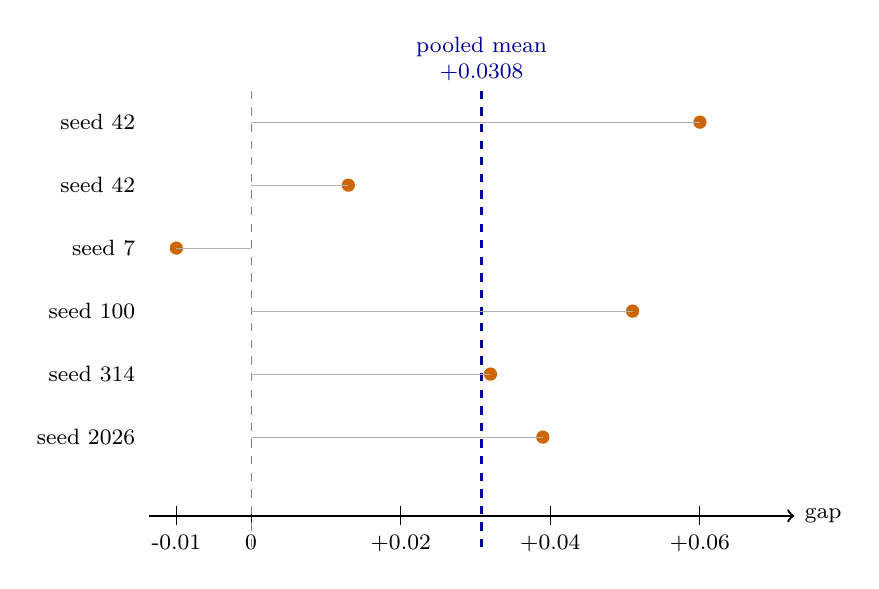
\begin{tikzpicture}[font=\footnotesize]
  % axes
  \def\xz{0}      % x origin
  \def\xs{95}     % x scale (per 0.01 gap) -- gaps range -0.01..0.06
  \draw[->, thick] (-1.3,0) -- (6.9,0) node[right] {gap};
  \foreach \g/\lab in {-0.01/-0.01, 0/0, 0.02/+0.02, 0.04/+0.04, 0.06/+0.06} {
    \draw ({\g*\xs},0.12) -- ({\g*\xs},-0.12) node[below] {\lab};
  }
  % zero reference line
  \draw[dashed, gray] (0,-0.4) -- (0,5.4);
  % pooled mean line
  \draw[thick, blue!60!black, dashed] ({0.0308*\xs},-0.4) -- ({0.0308*\xs},5.4);
  \node[blue!60!black, anchor=south, align=center] at ({0.0308*\xs},5.4)
    {pooled mean\\$+0.0308$};
  % runs (y from top to bottom)
  \foreach \y/\seed/\gap in {
      5/42/0.060,
      4.2/42/0.013,
      3.4/7/-0.010,
      2.6/100/0.051,
      1.8/314/0.032,
      1.0/2026/0.039} {
    \node[anchor=east] at (-1.35,\y) {seed \seed};
    \fill[orange!80!black] ({\gap*\xs},\y) circle (2.4pt);
    \draw[gray!60] (0,\y) -- ({\gap*\xs},\y);
  }
\end{tikzpicture}
\caption[Per-run GCA$-$Holistic accuracy gap at $n=1{,}000$]{Per-run GCA$-$Holistic accuracy gap at $n=1{,}000$, against the pooled
mean. Five of six runs favor GCA, but the spread across runs is wide relative to
the pooled effect, which is why no single run was treated as conclusive.}
\label{fig:per-run-gaps}
\end{figure}

\begin{table}[htbp]
\centering
\caption[Averaged result across six runs at $n=1{,}000$]{Averaged result across 6 runs / 30 cross-validation folds at
$n=1{,}000$. The interval and $p$-value are computed over folds, which are not
independent observations, and are therefore exploratory and anti-conservative
(Chapter~\ref{ch:methodology}, Section~\ref{sec:methodology-rm-eval}).}
\label{tab:pooled-headline}
\begin{tabular}{rrrrr}
\toprule
Holistic mean & GCA mean & Gap & 95\% fold-level CI & Fold-level Wilcoxon $p$ \\
\midrule
0.5295 & 0.5603 & \textbf{+0.0308} & $[+0.013, +0.047]$ & 0.0034 \\
\bottomrule
\end{tabular}
\end{table}

At the fold level, GCA leads in 22 of the 30 folds (73\%), with no ties. Both
conditions sit close to chance in absolute terms: 0.5295 and 0.5603 are 2.95
and 6.03 percentage points above the 0.5 chance level.

Table~\ref{tab:evidence-progression} tracks how the fold-level estimate changed
as runs were added. The interval narrows at each stage while the point estimate
stays near three percentage points, though the independence caveat of
Chapter~\ref{ch:methodology}, Section~\ref{sec:methodology-rm-eval} applies to
every row.

\begin{table}[htbp]
\centering
\caption[Progression of the pooled estimate as runs were added]{Progression of the pooled statistical estimate as runs were added. The
$p$-values are subject to the independence caveat discussed in
Chapter~\ref{ch:discussion}, Section~\ref{sec:disc-stats-caveat}.}
\label{tab:evidence-progression}
\begin{tabular}{lrrrrr}
\toprule
Stage & Runs & Folds & Pooled gap & 95\% CI & Wilcoxon $p$ \\
\midrule
Two-run  & 2 & 10 & $+0.034$ & $[+0.003, +0.064]$ & 0.084 \\
Five-run & 5 & 25 & $+0.029$ & $[+0.009, +0.048]$ & 0.0123 \\
Six-run  & 6 & 30 & $+0.031$ & $[+0.013, +0.047]$ & 0.0034 \\
\bottomrule
\end{tabular}
\end{table}

At six runs, the fold-pooled $p$-value had already fallen to 0.0034, yet the
run-level test could not fall below 0.0312 no matter how consistent the six runs
were, because that is the smallest two-sided value the Wilcoxon signed-rank test
can return with six paired observations; with five wins and one loss the
attainable minimum is 0.0625. The six-run campaign was therefore not merely
inconclusive by chance; it was structurally unable to establish run-level
significance at the conventional threshold, independent of the true size of the
effect. Resolving this required more runs, which in turn required the
reward-model training procedure to be fully deterministic under a given seed, a
property it did not previously have
(Chapter~\ref{ch:implementation}, Section~\ref{sec:impl-rm-training}).
